\documentclass[letter,twocolumn]{article}

\usepackage{geometry}
\geometry{
		total={7.5in,10in},
	}



\usepackage{graphics}
\usepackage{graphicx} % For including and formatting image files
\usepackage{multirow}
\usepackage{longtable}
\usepackage{epsfig}
\usepackage{epstopdf}

\usepackage{amsmath, mathrsfs, dsfont}
\usepackage{amssymb}
\usepackage{amsfonts}
\usepackage{amsbsy}
\usepackage{bm}


\usepackage{cite}
\usepackage{verbatim}

\usepackage{amscd}
\usepackage{color}
\definecolor{lgray}{gray}{0.6}
\usepackage{rotating}


%\usepackage[font=footnotesize]{caption}
%\usepackage[caption=false,font=footnotesize]{subfig}
\usepackage[font=footnotesize]{subcaption}

\usepackage{mathptmx}
\usepackage[11pt]{moresize}
\usepackage{flushend}
\usepackage[stable]{footmisc}

\usepackage{algorithmicx}
\usepackage{algorithm}
\usepackage{algpascal}
\usepackage{float}
\usepackage{algc}
\usepackage{algcompatible}
\usepackage{algpseudocode}

\renewcommand{\algorithmicrequire}{\textbf{Input:}}  % Use Input in the format of Algorithm  
\renewcommand{\algorithmicensure}{\textbf{Output:}} % Use Output in the format of Algorithm  
\usepackage[vcentermath]{youngtab} % For typesetting Young Tableaux
\usepackage{url}
%\usepackage{breakurl}   
            

%-----------------------------------------%
% Define custom symbols
\newcommand{\BoldA}				{ \mathbf{A} }
\newcommand{\Bolda}				{ \mathbf{a} }
\newcommand{\BoldB}				{ \mathbf{B} }
\newcommand{\Boldb}				{ \mathbf{b} }
\newcommand{\BoldC}				{ \mathbf{C} }
\newcommand{\Boldc}				{ \mathbf{c} }
\newcommand{\BoldD}				{ \mathbf{D} }
\newcommand{\Boldd}				{ \mathbf{d} }
\newcommand{\BoldE}				{ \mathbf{E} }
\newcommand{\Bolde}				{ \mathbf{e} }
\newcommand{\BoldF}				{ \mathbf{F} }
\newcommand{\Boldf}				{ \mathbf{f} }
\newcommand{\BoldG}				{ \mathbf{G} }
\newcommand{\g}					{ \mathbf{g} }
\newcommand{\BoldH}				{ \mathbf{H} }
\newcommand{\Boldh}				{ \mathbf{h} }
\newcommand{\BoldI}				{ \mathbf{I} }
\newcommand{\I}					{ \mathbf{I} }
\newcommand{\BoldJ}				{ \mathbf{J} }
\newcommand{\BoldK}				{ \mathbf{K} }
\newcommand{\Boldk}				{ \mathbf{k} }
\newcommand{\BoldM}				{ \mathbf{M} }
\newcommand{\BoldN}				{ \mathbf{N} }
\newcommand{\Boldn}				{ \mathbf{n} }
\newcommand{\BoldO}				{ \mathbf{O} }
\newcommand{\BoldP}				{ \mathbf{P} }
\newcommand{\Boldp}				{ \mathbf{p} }
\newcommand{\BoldQ}				{ \mathbf{Q} }
\newcommand{\Boldq}				{ \mathbf{q} }
\newcommand{\BoldR}				{ \mathbf{R} }
\newcommand{\R}					{ \mathbf{R} }
\newcommand{\Boldr}				{ \mathbf{r} }
\newcommand{\Bolds}				{ \mathbf{s} }
\newcommand{\BoldS}				{ \mathbf{S} }
\newcommand{\BoldT}				{ \mathbf{T} }
\newcommand{\BoldU}				{ \mathbf{U} }
\newcommand{\Boldu}				{ \mathbf{u} }
\newcommand{\BoldV}				{ \mathbf{V} }
\newcommand{\Boldv}				{ \mathbf{v} }
\newcommand{\Boldw}				{ \mathbf{w} }
\newcommand{\BoldW}				{ \mathbf{W} }
\newcommand{\BoldX}				{ \mathbf{X} }
\newcommand{\Boldx}				{ \mathbf{x} }
\newcommand{\BoldY}				{ \mathbf{Y} }
\newcommand{\Boldy}				{ \mathbf{y} }
\newcommand{\BoldZ}				{ \mathbf{Z} }
\newcommand{\Boldz}				{ \mathbf{z} }


\newcommand{\0}					{ \boldsymbol{0} }
\newcommand{\1}					{ \boldsymbol{1} }

\newcommand{\dtheta}			{ \delta\boldsymbol{\theta} }
\newcommand{\noiseg}			{ \mathbf{n}_{g} }
\newcommand{\noisewg}			{ \mathbf{n}_{{\omega}g} }
\newcommand{\noisea}			{ \mathbf{n}_{a} }
\newcommand{\noisewa}			{ \mathbf{n}_{{\omega}a} }
\newcommand{\Boldomega}			{ \boldsymbol{\omega} }
\newcommand{\Boldnu}			{ \boldsymbol{\nu} }
\newcommand{\BoldGamma}			{ \boldsymbol{\Gamma} }
\newcommand{\Boldgamma}			{ \boldsymbol{\gamma} }
\newcommand{\Boldkappa}			{ \boldsymbol{\kappa} }
\newcommand{\BoldPhi}			{ \boldsymbol{\Phi} }
\newcommand{\Boldphi}			{ \boldsymbol{\phi} }
\newcommand{\Boldpi}			{ \boldsymbol{\pi} }
\newcommand{\Boldrho}			{ \boldsymbol{\rho} }
\newcommand{\Boldell}			{ \boldsymbol{\ell} }
%\newcommand{\0}					{ \boldsymbol{0} }
\newcommand{\Bolddelta}			{ \boldsymbol{\delta} }
\newcommand{\BoldDelta}			{ \boldsymbol{\Delta} }
\newcommand{\BoldTheta}			{ \boldsymbol{\Theta} }
\newcommand{\Boldtheta}			{ \boldsymbol{\theta} }
\newcommand{\BoldSigma}			{ \boldsymbol{\Sigma} }
\newcommand{\Boldsigma}			{ \boldsymbol{\sigma} }
\newcommand{\Boldeps}			{ \boldsymbol{\epsilon} }
\newcommand{\Boldmu}			{ \boldsymbol{\mu} }
\newcommand{\Boldeta}			{ \boldsymbol{\eta} }
\newcommand{\Boldzeta}			{ \boldsymbol{\zeta} }
\newcommand{\Boldlambda}		{ \boldsymbol{\lambda} }
\newcommand{\BoldLambda}		{ \boldsymbol{\Lambda} }
\newcommand{\Boldchi}			{ \boldsymbol{\chi} }

\newcommand{\E}					{\mathrm{E}}
\newcommand{\Var}				{\mathrm{Var}}
\newcommand{\Cov}				{\mathrm{Cov}}
\newcommand\norm[1]{\lVert#1\rVert}

\newcommand\T{\rule{0pt}{2.6ex}}       % Top strut
\newcommand\B{\rule[-1.2ex]{0pt}{0pt}} % Bottom strut

\newcounter{inlineenum}
\renewcommand{\theinlineenum}{\alph{inlineenum}}
\newenvironment{inlineenum}
{\unskip\ignorespaces\setcounter{inlineenum}{0}%
	\renewcommand{\item}{\refstepcounter{inlineenum}{\textit{\theinlineenum})~}}}

\newcommand{\icol}[1]{% inline column vector
	\left(\begin{matrix}#1\end{matrix}\right)%
}
\newcommand{\irow}[1]{% inline row vector
	\begin{matrix}(#1)\end{matrix}%
}

%-----------------------------------------%
% Define custom operators
\DeclareMathOperator*{\argmin}{\emph{arg\,min}}
\DeclareMathAlphabet{\mathcal}{OMS}{cmsy}{m}{n}

%-----------------------------------------%
% Define custom commands
%\newcommand{\or}{\bf or}
%\newcommand{\and}{\bf and}
\newtheorem{Theorem}{Theorem}[section]
\newtheorem{Proposition}[Theorem]{Proposition}
\newtheorem{Lemma}[Theorem]{Lemma}
\newtheorem{Corollary}[Theorem]{Corollary}
\newtheorem{Remark}[Theorem]{\textbf{Remark}}
	\newcommand{\brmrk}[1]{\begin{remark} \label{#1} }
	\newcommand{\ermrk}{ \hfill $\bigtriangleup$    \end{remark} \vspace{1mm} }
\newtheorem{Definition}[Theorem]{Definition}
\newtheorem{Example}[Theorem]{Example}
\newtheorem{Conjecture}[Theorem]{Conjecture}
\newtheorem{Problem}[Theorem]{Problem}
\newtheorem{Algorithm}[Theorem]{Algorithm}
\newtheorem{CardGame}[Theorem]{Card Game}
\newtheorem{Strategy}[Theorem]{Strategy}
\newtheorem{Question}[Theorem]{Question}
\newtheorem{exercise}{Exercise}[section]
\newcommand{\boex}[1]{\begin{example} \label{#1} --- \rm}
	\newcommand{\eoex}{ \hfill $\bigtriangleup$    \end{example} \vspace{1mm} }
\newtheorem{example}{Example}[section]
\newcommand{\bohw}[1]{\begin{exercise} \label{#1} -- \rm}
	\newcommand{\eohw}{ \hfill    \end{exercise} \vspace{1mm} }
\newtheorem{assumption}{Assumption}[section]
	\newcommand{\boass}[1]{\begin{assumption} \label{#1} -- \rm}
	\newcommand{\eoass}{ \hfill    \end{assumption} \vspace{1mm} }

\newcommand{\todo}[1]{\footnote{\color{green}TO DO: {#1}}}

\newcommand{\tstamp}{\today}
%\usepackage{fancyhdr}
%\pagestyle{fancy}
%\headheight 35pt

%\rhead{\tstamp}
%\chead{Middle top}
%\lhead{Left top}
%\rfoot{p. \thepage}
%\cfoot{}
%\lfoot{Copyright \textcopyright 2019, University of California, Riverside. All Rights reserved.}

\renewcommand{\baselinestretch}{1.0}

\setcounter{secnumdepth}{3}
\setcounter{tocdepth}{2}

\newcommand{\black}{\color{black}}
\newcommand{\blue}{\color{blue}}
\newcommand{\red}{\color{red}}
\newcommand{\green}{\color{green}}
\newcommand{\magenta}{\color{magenta}}
\newcommand{\cyan}{\color{cyan}}
\newcommand{\orange}{\color{orange}}
\definecolor{brinkpink}{rgb}{1.00, 0.33, 0.64}
\newcommand{\pink}{\color{brinkpink}}

%\newcommand{\black}{\color{black}}
%\newcommand{\blue}{\color{black}}
%\newcommand{\red}{\color{black}}
%\newcommand{\green}{\color{black}}
%\newcommand{\magenta}{\color{black}}

\makeatletter
\newenvironment{breakablealgorithm}
{% \begin{breakablealgorithm}
	\begin{center}
		\refstepcounter{algorithm}% New algorithm
		\hrule height.8pt depth0pt \kern2pt% \@fs@pre for \@fs@ruled
		\renewcommand{\caption}[2][\relax]{% Make a new \caption
			{\raggedright\textbf{\ALG@name~\thealgorithm} ##2\par}%
			\ifx\relax##1\relax % #1 is \relax
			\addcontentsline{loa}{algorithm}{\protect\numberline{\thealgorithm}##2}%
			\else % #1 is not \relax
			\addcontentsline{loa}{algorithm}{\protect\numberline{\thealgorithm}##1}%
			\fi
			\kern2pt\hrule\kern2pt
		}
	}{% \end{breakablealgorithm}
		\kern2pt\hrule\relax% \@fs@post for \@fs@ruled
	\end{center}
}
\makeatother







 

\begin{document}
	\title{ASD to State-Space Example: Sample Notebook Result}
\author{Jay~A.~Farrell}
\maketitle

\begin{abstract}
This article presents and discusses example results generated using the Python Jupyter notebook:
\begin{verbatim}
	Demo_FirstOrderGM_AccelMarbleSlab.ipynb
\end{verbatim}
It should exist in the same repository as this pdf file. 

Before running the notebook, unzip the file:
\begin{verbatim}
parsed_isolated_marble_data_az.zip
\end{verbatim} 
in the AV\_Matlab\_SW\_IEEECSM directory,
to extract the parsed\_isolated\_marble\_data\_az.mat file.
The results herein were produced using the following parameter settings: 
\begin{itemize}
	\item sample frequency $Fs = 100$ Hz,
	\item velocity random walk $N  = 3.3e-3$ m/s/s/rtHz = m/s/rtsec,
	\item bias instability $B  = 9e-4$ m/s/s,
	\item desired delay for the Gauss-Markov ASD peak $T_p = 300$ sec.,
	\item state-space simulation duration 10e3 sec. (1e6 samples),
	\item covariance test average time $T\_avg = 10$ seconds, and
	\item covariance test integration time $T\_int = 20$ seconds.
\end{itemize}
\end{abstract}

\section{Problem Setup}
The blue dots in Fig. \ref{fig:ASD_plot} show samples of the Allan Standard Deviation (ASD) curve for an accelerometer for delays $\tau\in[0.01, 500]$ seconds.


The optimal estimator that we are building requires a finite-dimensional, discrete-time, state-space model for the stochastic error in each IMU output.
The model for each output has the form:
\begin{align}
	\Boldx(k+1) &= \BoldPhi\, \Boldx(k) + \BoldGamma \, \Boldomega(k) \\
	z(k)   &= \BoldC \,  \Boldx(k) + \nu(k),
\end{align}
where $\Boldx\in\Re^n$, $z(k)$ is scalar, and the matrices have appropriate dimensions. 
Both $\Boldomega\sim N(\0,\BoldQ_\omega)$ and $\nu\sim N(0,Q_\nu)$ are white and Gaussian. 
The goal is to specify the model parameters: $n$, $\BoldPhi$, $\BoldGamma$, $\BoldC$, $\BoldQ_\omega$, and $Q_\nu$.

There is no finite-dimensional model that can match the ASD curve for all delays $\tau$.
The approximate fit to the curve can be improved by increasing $n$; however \cite{CSM_IMU}:
\begin{itemize}
	\item The computational load increase with the cube of the number of states in the estimator. Because the IMU has six out puts, six error models are required, so the selection of $n$ has computation impact proportional to $(6\, n)^3.$
	\item Adding states can have a negative impact on observability that can negatively impact performance.
\end{itemize} 
The purpose of the state-space model is to communicate to the estimator the magnitude and correlation properties 
of the IMU output stochastic error sequence over the time intervals relevant to the estimator. 
The lowest order state-space model that can do the job should be selected.


\section{Specifications}
For this example the goal is to approximately match the ASD graph for delays $\tau\in[T_s, 100]$ seconds, where $T_s = \frac{1}{F_s}$. This range is selected because the INS approach will integrate at 100Hs and is expected to receive aiding signals at one Hertz with gaps between measurements not to exceed 10 s. 
If aiding measurements are absent for greater than 10s, the propagated covariance will still reflect the accuracy of the navigation for several 10's of seconds while other actions take place. 


\begin{figure}[tbh]
	\centering
	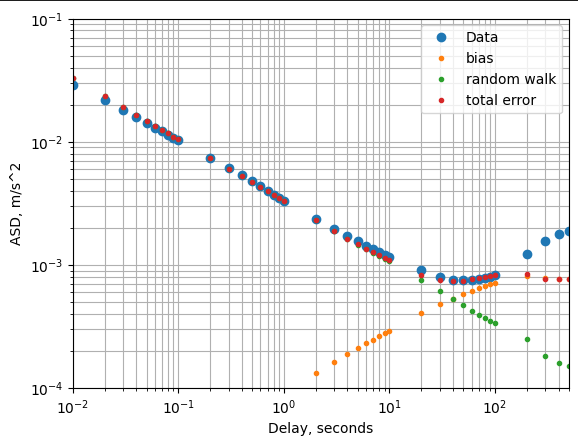
\includegraphics[trim=0in 0in 0in 0.1in, clip, width=0.9\columnwidth]{figure/ASD_plot}
	\caption{Allan Standard Deviation Plot.}
	\label{fig:ASD_plot}
\end{figure}

\section{Selection of AV Parameters}
The value of $N$ is read from the ASD graph as the value at $\tau = 1$ second: $N= 3.3e-3$ m/s/s/rtHz = m/s/rtsec. The method to compute $Q_\nu$ from $N$ are documented in the python code.  


This example will use a state-space model order $n=1$ where the single state element will be denoted by $b$ and referred to as a bias. The model has simplifies to 
\begin{align}
	b(k+1) &= \mu\, b(k) + \omega(k) \\
	z(k)   &= b(k) + \nu(k).
\end{align}
The method to compute the  model parameters $\mu$ and $Q_\omega$ based on the choice of the bias instability parameter $B$ and the parameter $T_p$ are documented in the python code. The values of $B$ and the parameter $T_p$ are adjusted manually to achieve the desired ASD shape in the region where the curve flattens. 
For the present example, the bias instability parameter is selected as
$B  = 9.0e-4$ m/s/s
and the desired delay at which the ASD plot of the Gauss-Markov model should have its peak is
$Tp = 300$  seconds.

\section{Results}
The Jupyter notebook outputs the following:
\begin{itemize}
	\item 
	Continuous-time model is (units depend on context): \\
	z(t) = b(t) + n(t), \\
	db(t)/dt = -6.3000e-03 * b(t) + w(t), \\
	where n(t) is white noise with PSD $Sn = 1.0890e-05$
	and w(t) is the bias process noise with PSD $Sw = 2.6783e-08$
	The steady-state covariance of the bias process is Pb\_ss\_c = 2.1256e-06.
	
	\item Discrete-time model is (units depend on context): \\
	z[k] = b[k] + n[k], \\
	b[k+1] = 0.9999 * b[k] + w[k], \\
	where n[k] is white noise with covariance Qn = 1.0890e-03 (std 3.3000e-02)
	and w[k] is the bias process with covariance Qw = 2.6781e-10 (std 1.6365e-05).
	The steady-state covariance of the bias process is Pb\_ss\_d = 2.1256e-06.
\end{itemize}
Note that both models have the same steady-state covariance for the bias.

The discrete-time model is easily simulated to yield data sequences that can be used to check the validity of the error model.


\begin{figure}[bth]
	\centering
	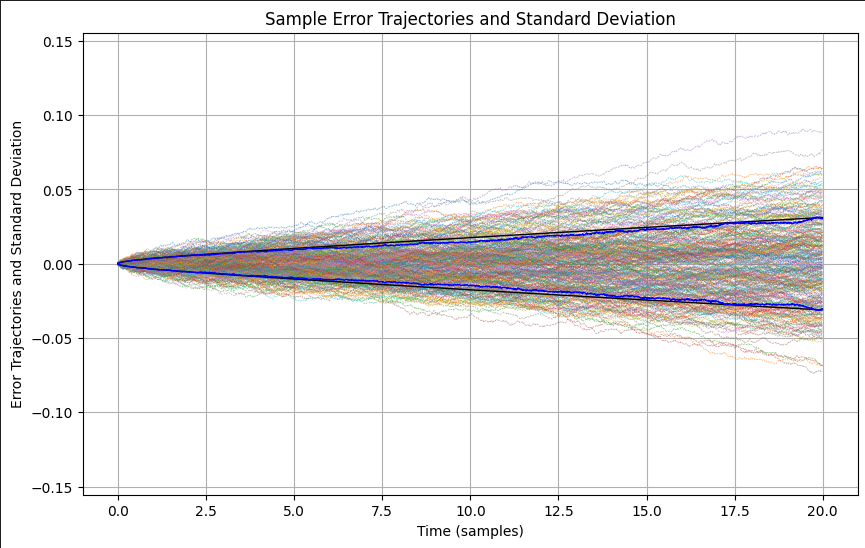
\includegraphics[trim=0.1in 0in 0in 0.1in, clip, width=\columnwidth]{figure/cov_sim}
	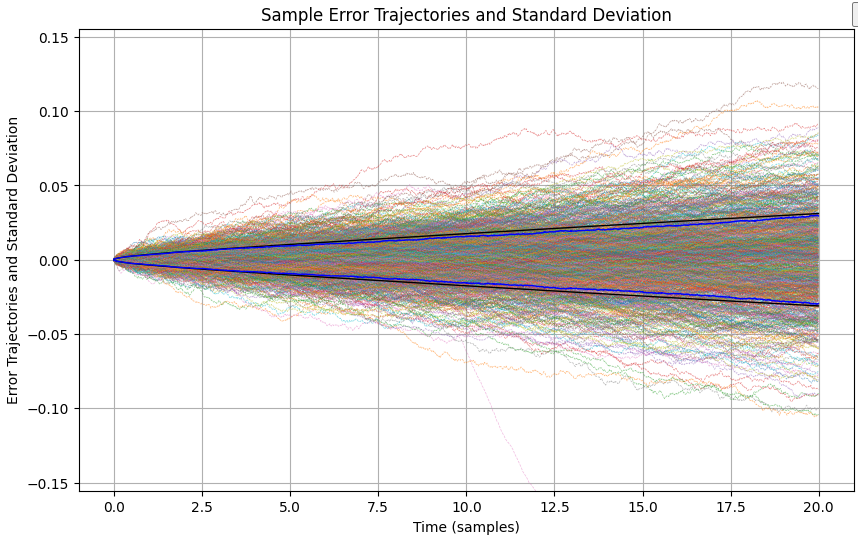
\includegraphics[trim=0in 0in 0in 0.01in, clip, width=\columnwidth]{figure/cov_instrument}
	\caption{Covariance Check Graphs. 
		Top: One thousand sample error trajectories computed by integrating the output of the state-space error model. 
		Bottom: One thousand sample error trajectories computed by integrating the IMU data after subtracting a prior estimate of the bias.
		Black solid curve is the theoretical standard deviation from the state-space model. 
		Blue solid curve is the sample standard deviation at each time instant over the sample trajectories. }
	\label{fig:cov_plot}
\end{figure}


\subsection{Check: ASD Plot}
Fig. \ref{fig:ASD_plot} shows the ASD graph for the simulate output of the state-space error model as red dots. These closely match the ASD plot for the instrument data for $tau\in[T_s,100]$ seconds. 

The figure also shows the ASD plot for both components $b$ (orange)and $\nu$ (green) that are summed to create the overall output $z$. The value of $B$ was selected to get the appropriate height of the the ASD for $b$ and the value of $T_p$ was adjusted so that the overall plot had the desired shape for $\tau\in[10,100]$ seconds.

\subsection{Check: Covariance}
The main purpose of the model is to communicate to the optimal estimation routine the magnitude and correlation structure of the IMU errors. The IMU outputs are integrated to produce angles or velocities. 

Therefore, this section compares the growth of the growth of the integrated error in a few ways:
\begin{itemize}
	\item The error model produces 1000 simulated integrated error trajectories. 
	Each is plotted as a narrow opaque curve in the top portion of Fig. \ref{fig:cov_plot}. 
	At each time instant the robust standard deviation is computed and plotted as a blue line.
	The theoretical error covariance is computed using the state-space model and eqn. (4.125) in \cite{farrell2008aided}. 
	This is plotted as the black line. 
	Note that the blue and black lines match closely at all times.
	\item 	After removing a constant prior estimate of the bias, the instrument data produces 1000 simulated integrated error trajectories. 
	Each is plotted as a narrow opaque curve in the bottom portion of Fig. \ref{fig:cov_plot}. 
	At each time instant the robust standard deviation is computed and plotted as a blue line.
	The theoretical error covariance is computed using the state-space model and eqn. (4.125) in \cite{farrell2008aided}. 
	This is plotted as the black line. 
	Note that the blue and black lines match closely at all times.
\end{itemize}


\bibliographystyle{IEEEtran}
\bibliography{refs.bib}
\end{document}